%! TEX program = lualatex
\documentclass[12pt,a4paper]{article} 

% Packages for formatting
\usepackage{fontspec}
\usepackage[ngerman]{babel}
\usepackage{geometry} 
\geometry{margin=1in} 
\usepackage{setspace} 
\usepackage{hyperref} 
\usepackage{xcolor}
\usepackage{amsmath} % for align*
\usepackage{amsthm} % neue Theorem-Umgebungen
\usepackage{enumitem} % für schöne Listen (Teilaufgaben)
\usepackage{mathbbol}
\usepackage{graphicx}
\usepackage{amssymb}
\usepackage{gensymb}

% Style settings
%\pagecolor{darkgray}      % sets background color to black 
%\color{gray}          % sets text color to white

% Change subsection to use a, b, c instead of 1, 2, 3
\renewcommand{\thesubsection}{\alph{subsection})}

% Title page info 
\title{Blatt 05}
\author{Hannes Rall \\ Albert-Ludwigs-University}
\date{\today}

\begin{document}
% Title page 
\begin{titlepage}
    \centering
    \vspace*{2cm}
    {\Huge\itshape Blatt 05\par}
    \vspace{2cm}
    {\Large\textsc{Hannes Rall}\par}
    \vfill
    {\large Albert-Ludwigs-University\\}
    \vspace{1cm}
    {\large\today\par}
\end{titlepage}

\newpage
\section*{Aufgabe 13}
\subsection*{(i)}
\begin{figure}[htbp]
    \centering        
    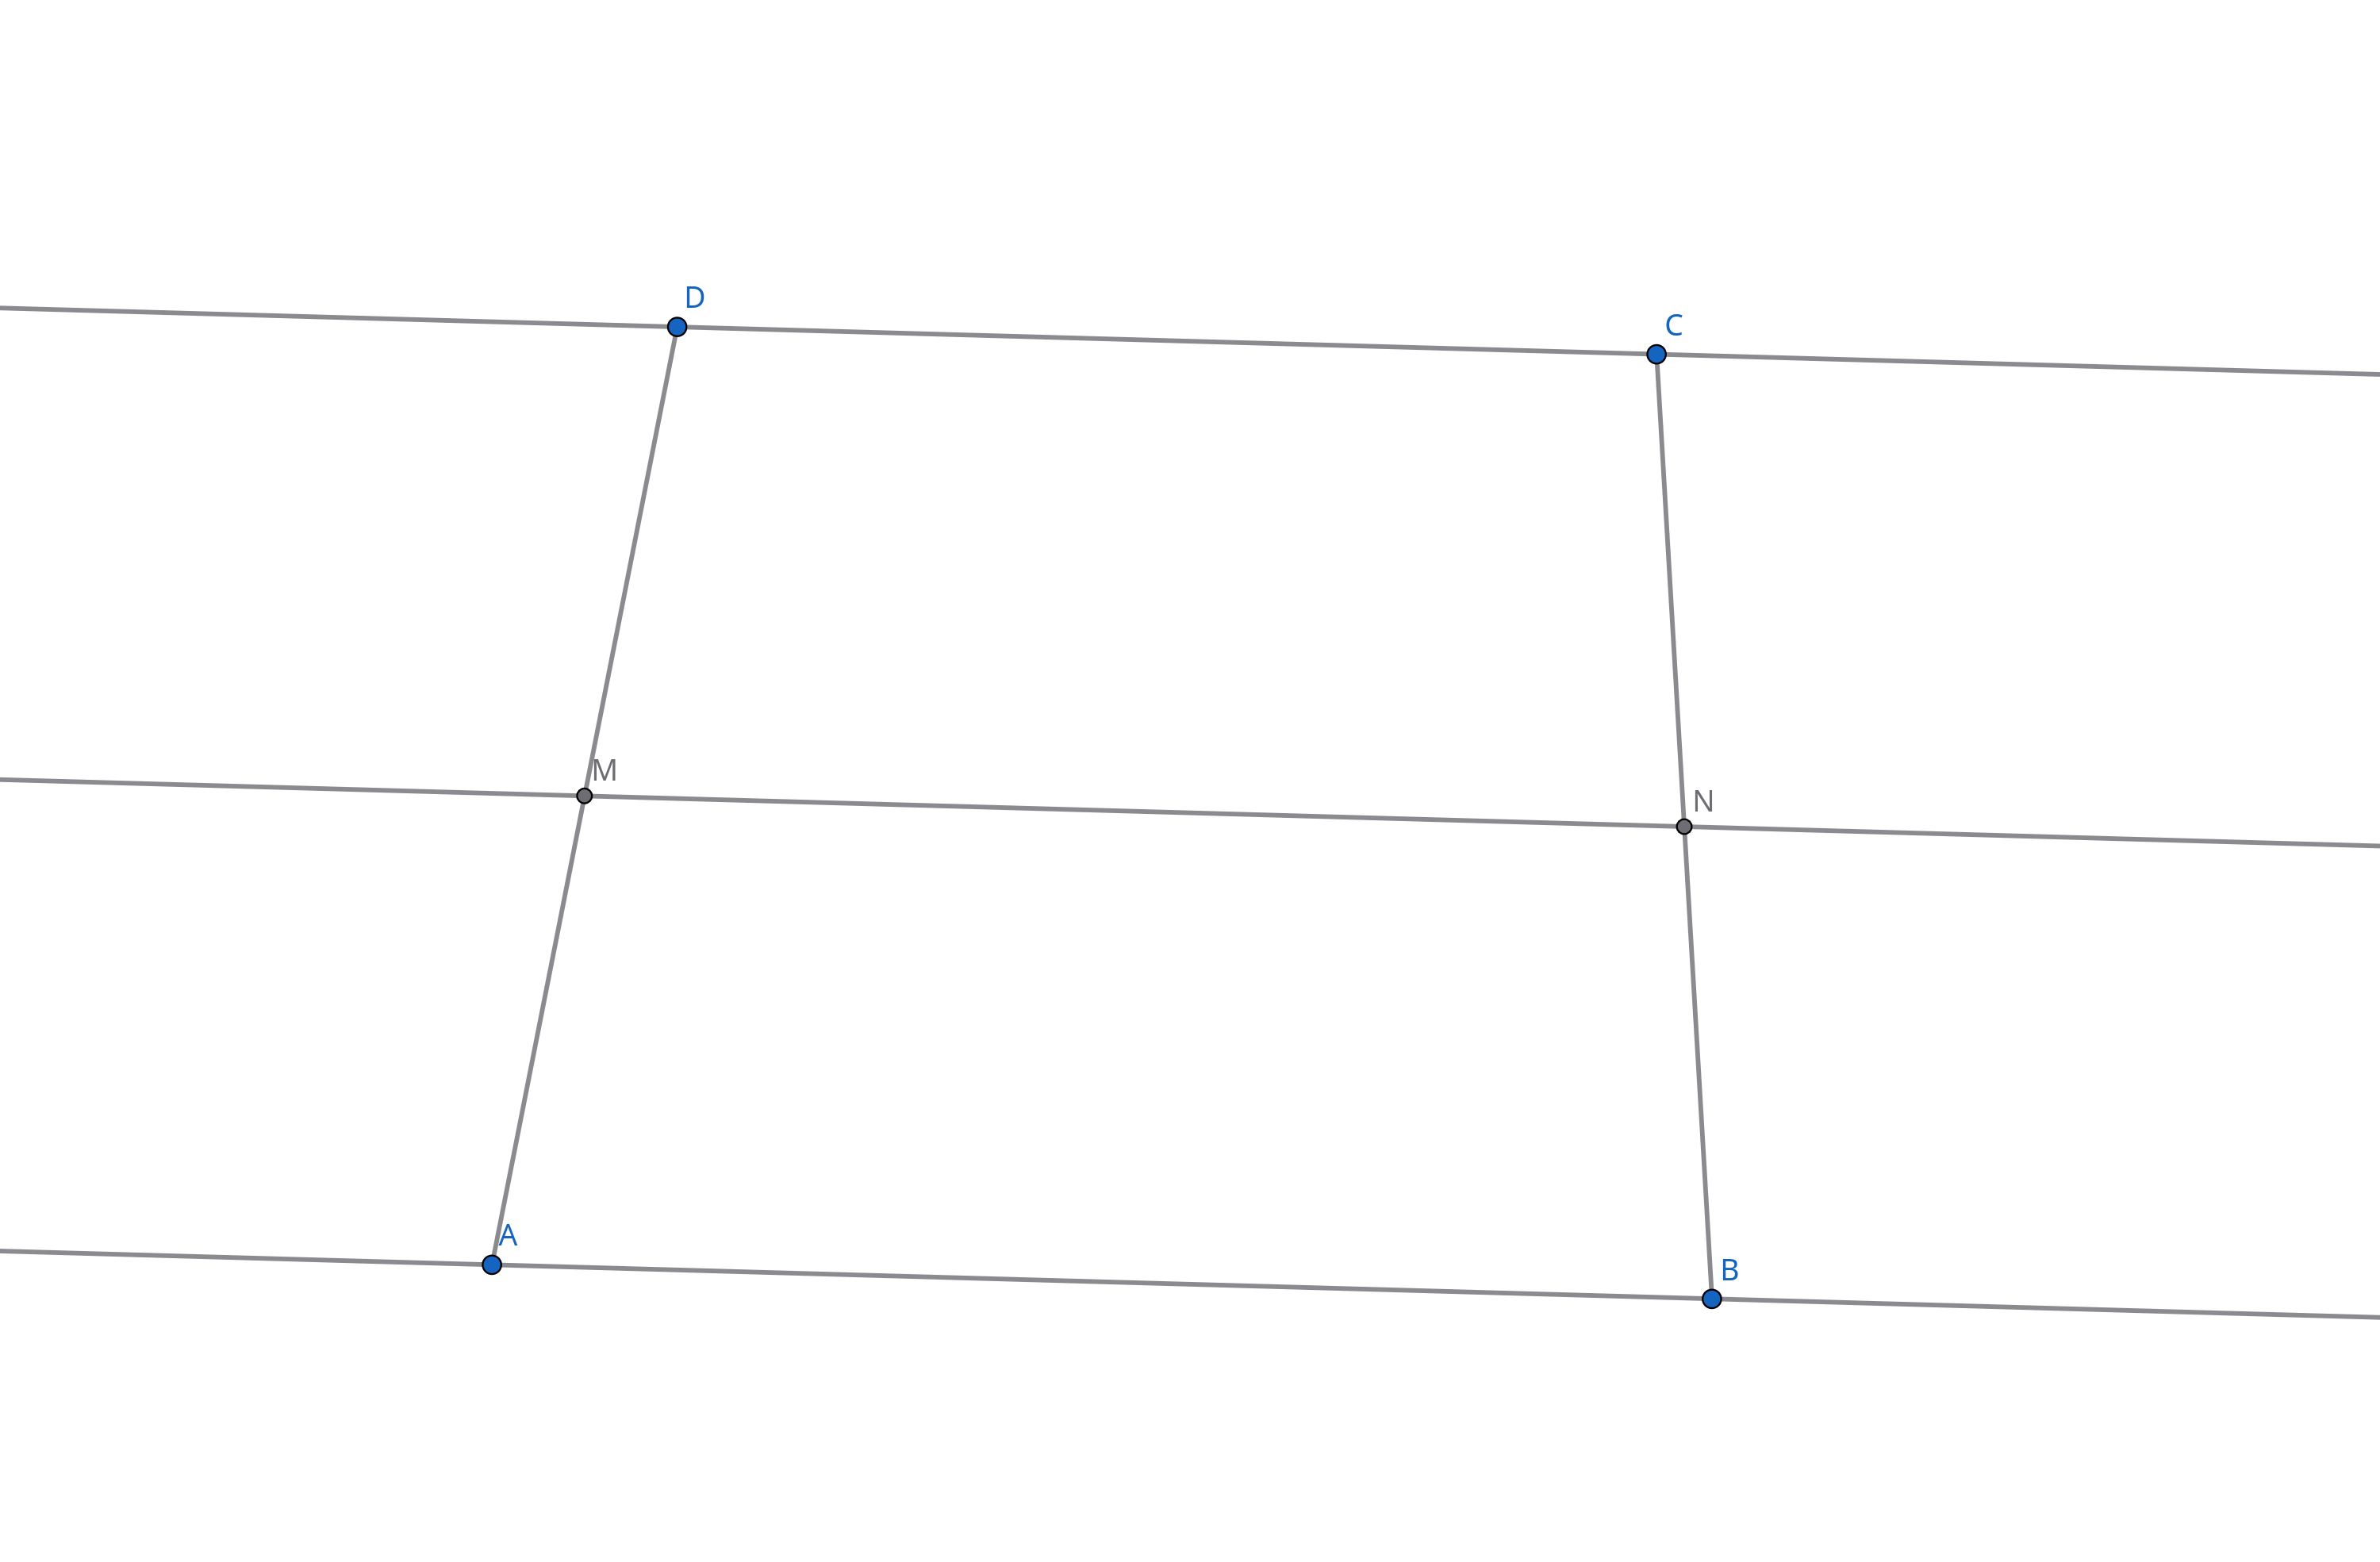
\includegraphics[width=0.8\textwidth]{Blatt05_Aufgabe_13_i.png}
    \caption{Skizze}
    \label{fig:mein_bild}
\end{figure}
\noindent Seien A, B, C und D Punkte. Wir betracheten das Trapez ABCD. Sei M der Mittelpunkt von $\overline{AD}$ und sei N der Mittelpunkt von $\overline{CD}$.
Es ist: \\
\[
    M = \frac{A + D}{2} \;\text{und}\; N = \frac{B+C}{2}
\]
Der Vektor $\overrightarrow{MN}$ ist: \\
\begin{align*}
    \overrightarrow{MN} &= N - M = \frac{B+C}{2} - \frac{A + D}{2} = \frac{(B-A) + (C-D)}{2} \\
                        &= \frac{\overrightarrow{AB} + \overrightarrow{DC}}{2}
\end{align*}
Da $g_{AB} \parallel g_{DC}$ gibt es ein $\lambda \in \mathbb{R}$, sodass
\[
    \lambda \cdot \overrightarrow{AB} = \overrightarrow{DC}
\]
Dann ist auch
\[
    \overrightarrow{MN} = \frac{(\lambda + 1)}{2} \overrightarrow{AB}
\]
Daraus folgt: $g_{MN} \parallel g_{AB}$.

\newpage
\subsection*{(ii)}

\newpage
\section*{Aufgabe 14}
\begin{figure}[htbp]
    \centering        
    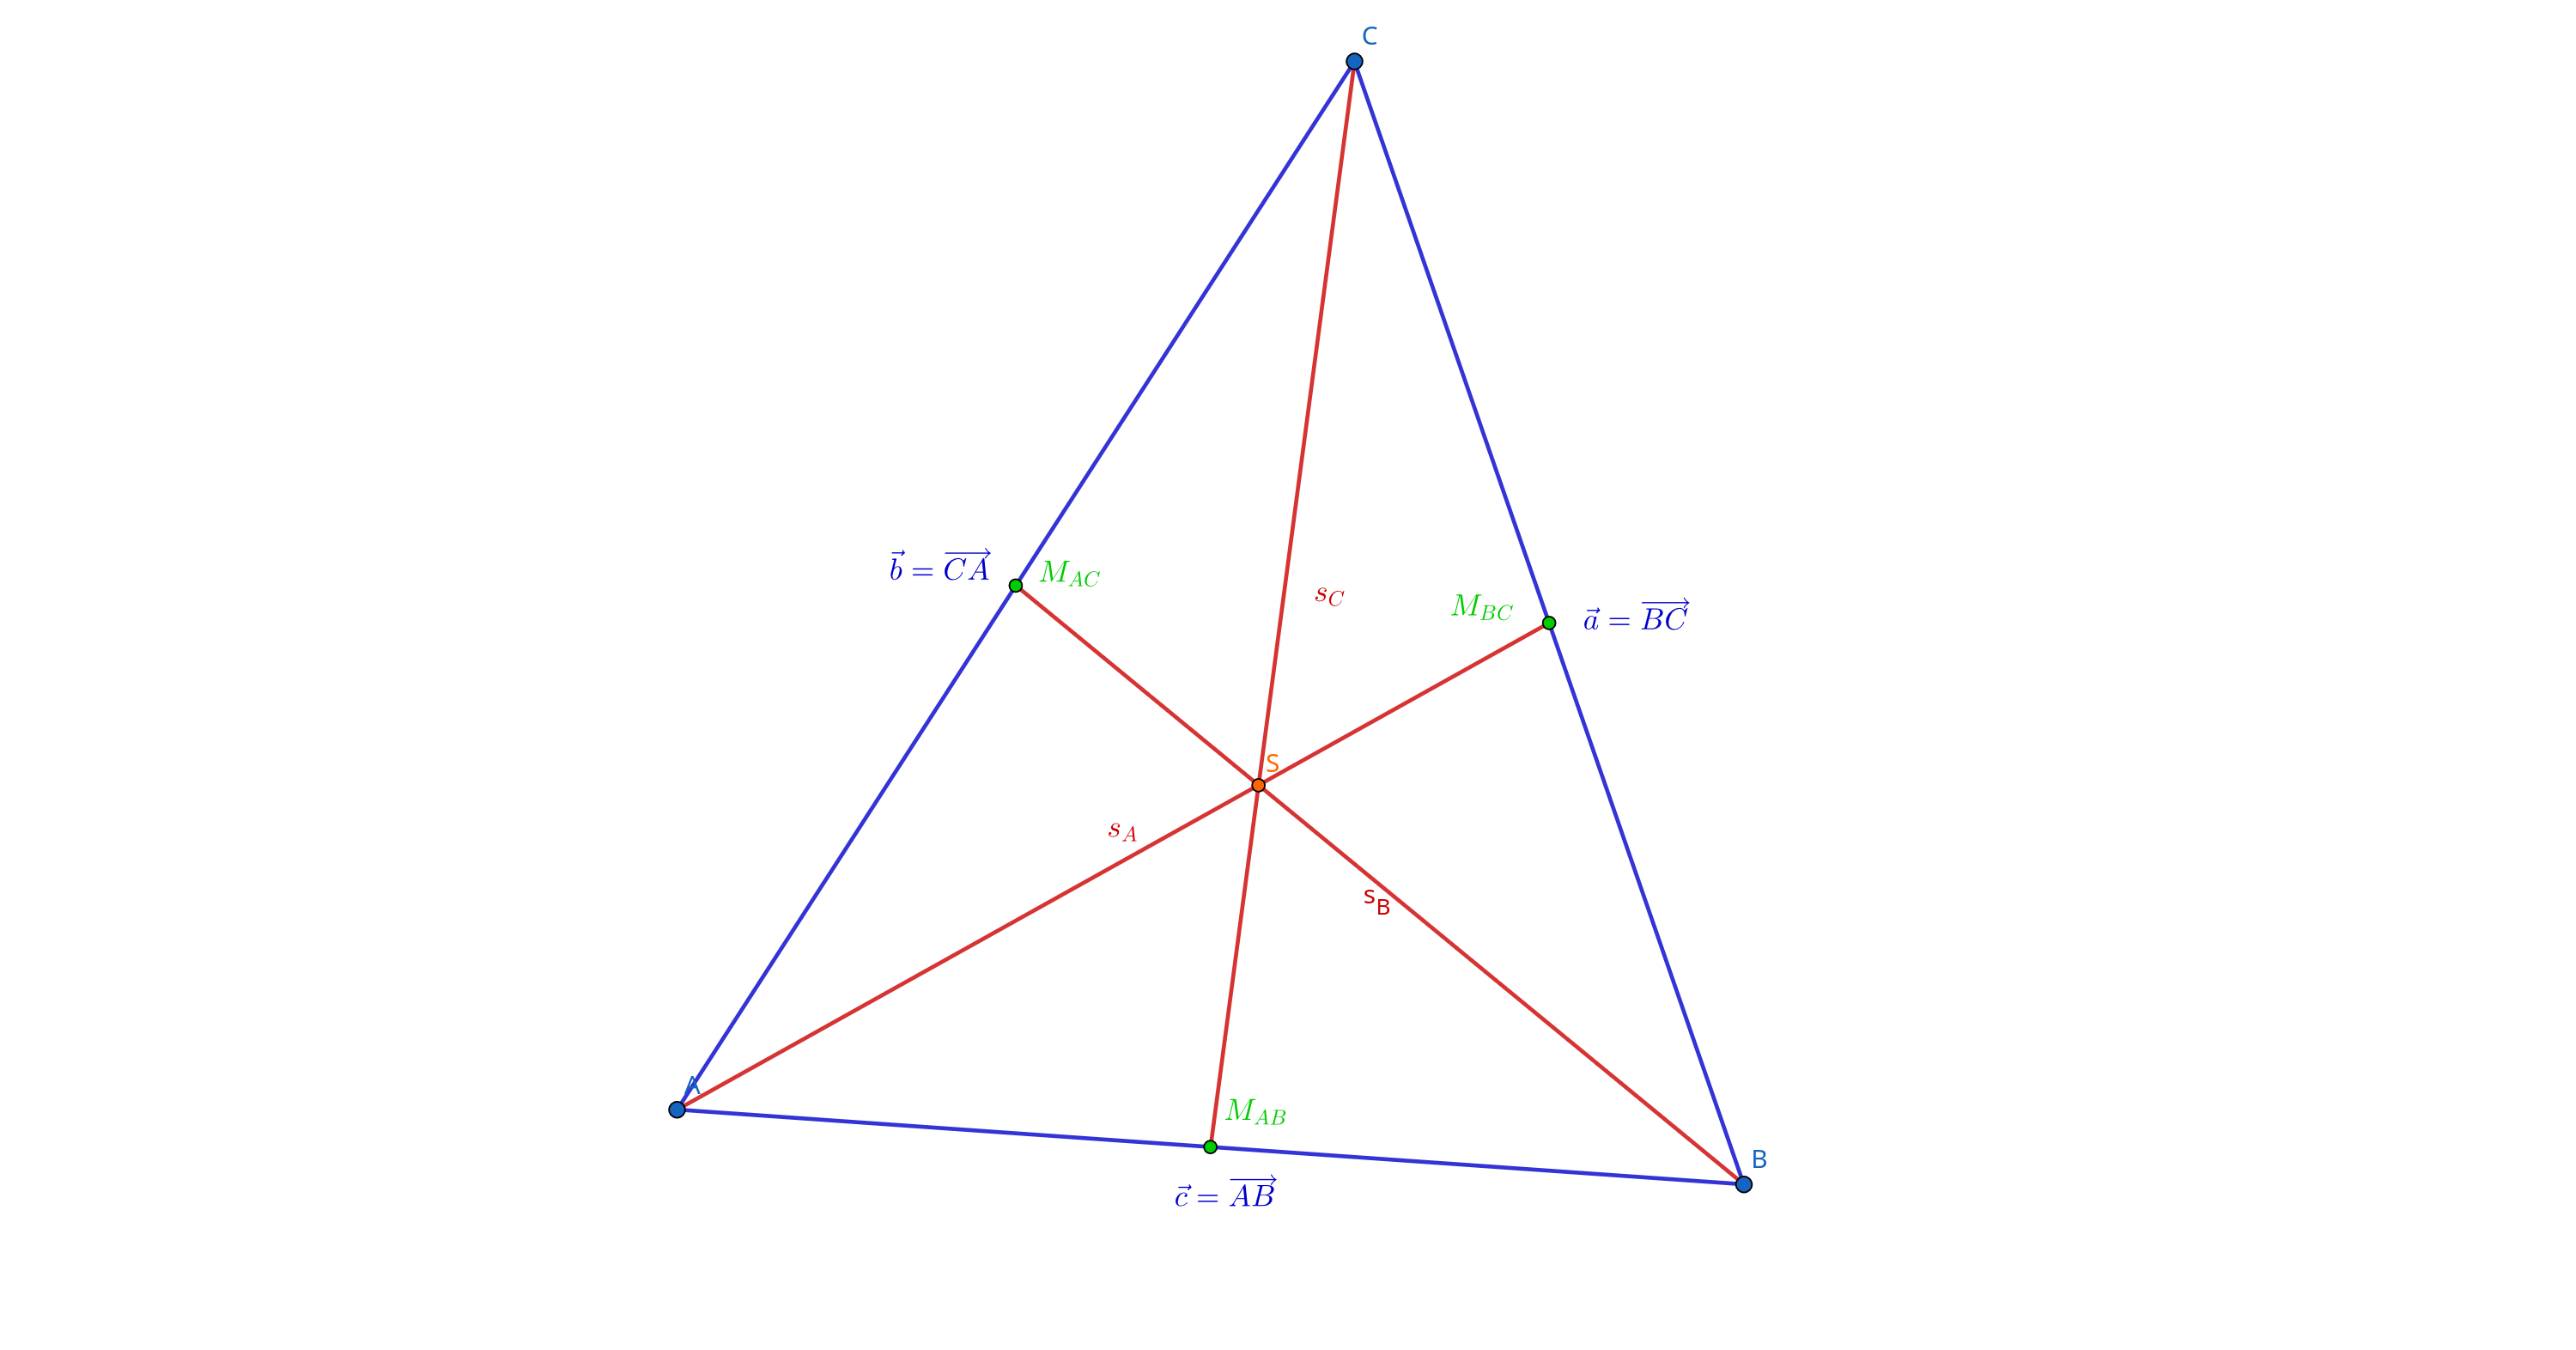
\includegraphics[width=0.8\textwidth]{Blatt05_Aufgabe_14.png}
    \caption{Skizze}
    \label{fig:mein_bild}
\end{figure}
\noindent Sei $\triangle ABC$ ein beliebiges Dreieck mit den Ortsvektoren $\overrightarrow{0A}$, $\overrightarrow{0B}$ und $\overrightarrow{0C}$.\\ 
Seien $M_{AB}$, $M_{BC}$ und $M_{AC}$ die Mittelpunkte der Seiten $AB$, $BC$ und $AC$: 
\[ 
    \overrightarrow{0M_{AB}} = \frac{1}{2}(\overrightarrow{0A} + \overrightarrow{0B}), \quad \overrightarrow{0M_{BC}} = \frac{1}{2}(\overrightarrow{0B} + \overrightarrow{0C}), \quad \overrightarrow{0M_{AC}} = \frac{1}{2}(\overrightarrow{0A} + \overrightarrow{0C}) 
\] 
Die Seitenhalbierende $s_C$ verläuft von $C$ zu $M_{AB}$, die Seitenhalbierende $s_B$ von $B$ zu $M_{AC}$. Wir suchen den Schnittpunkt $S$ dieser beiden Seitenhalbierenden. \\ 
\textbf{Parameterdarstellungen:} 
\begin{align*} 
    \text{Für } s_C: \quad \overrightarrow{0S}_C(t) &= \overrightarrow{0C} + t\left(\overrightarrow{0M_{AB}} - \overrightarrow{0C}\right) \\ 
                                                    &= \overrightarrow{0C} + t\left(\frac{1}{2}(\overrightarrow{0A} + \overrightarrow{0B}) - \overrightarrow{0C}\right) \\ 
                                                    &= (1-t)\overrightarrow{0C} + \frac{t}{2}\overrightarrow{0A} + \frac{t}{2}\overrightarrow{0B} 
\end{align*} 

\begin{align*} 
    \text{Für } s_B: \quad \overrightarrow{0S}_B(u) &= \overrightarrow{0B} + u\left(\overrightarrow{0M_{AC}} - \overrightarrow{0B}\right) \\ 
                                                    &= \overrightarrow{0B} + u\left(\frac{1}{2}(\overrightarrow{0A} + \overrightarrow{0C}) - \overrightarrow{0B}\right) \\ 
                                                    &= (1-u)\overrightarrow{0B} + \frac{u}{2}\overrightarrow{0A} + \frac{u}{2}\overrightarrow{0C} 
\end{align*}
\newpage
\noindent \textbf{Schnittpunkt:}\\
Setze $\overrightarrow{0S}_C(t) = \overrightarrow{0S}_B(u)$: 
\[ 
    (1-t)\overrightarrow{0C} + \frac{t}{2}\overrightarrow{0A} + \frac{t}{2}\overrightarrow{0B} = (1-u)\overrightarrow{0B} + \frac{u}{2}\overrightarrow{0A} + \frac{u}{2}\overrightarrow{0C} 
\] 
Vergleiche die Koeffizienten: 
\begin{align*} 
    \overrightarrow{0A}: &\quad \frac{t}{2} = \frac{u}{2} \implies t = u \\ \overrightarrow{0B}: &\quad \frac{t}{2} = 1-u \\ 
    \overrightarrow{0C}: &\quad 1-t = \frac{u}{2} 
\end{align*} 
Setze $t = u$ in die anderen Gleichungen: 
\begin{align*} 
    \frac{t}{2} &= 1-t \implies t + 2t = 2 \implies 3t = 2 \implies t = \frac{2}{3} \\ 
    1-t &= \frac{t}{2} \implies 2-2t = t \implies 2 = 3t \implies t = \frac{2}{3} 
\end{align*} 
\textbf{Einsetzen in die Parameterdarstellung:} 
\begin{align*} 
    \overrightarrow{0S} &= (1-t)\overrightarrow{0C} + \frac{t}{2}\overrightarrow{0A} + \frac{t}{2}\overrightarrow{0B} \\ 
                        &= \left(1 - \frac{2}{3}\right)\overrightarrow{0C} + \frac{1}{3}\overrightarrow{0A} + \frac{1}{3}\overrightarrow{0B} \\ 
                        &= \frac{1}{3}\overrightarrow{0C} + \frac{1}{3}\overrightarrow{0A} + \frac{1}{3}\overrightarrow{0B} 
\end{align*} 
\textbf{Verhältnis:}\\ 
Da $t = \frac{2}{3}$, teilt der Schwerpunkt $S$ die Seitenhalbierende $s_C$ im Verhältnis $2:1$ (vom Eckpunkt $C$ aus gezählt). \\ 
\textbf{Folgerung:}\\ Da dies für jede Seitenhalbierende gilt (also die Argumentation ist o.B.d.A.), schneiden sich alle drei Seitenhalbierenden in einem Punkt, dem Schwerpunkt, und dieser teilt jede Seitenhalbierende im Verhältnis $2:1$.

\newpage
\section*{Aufgabe 15}
\begin{figure}[htbp]
    \centering        
    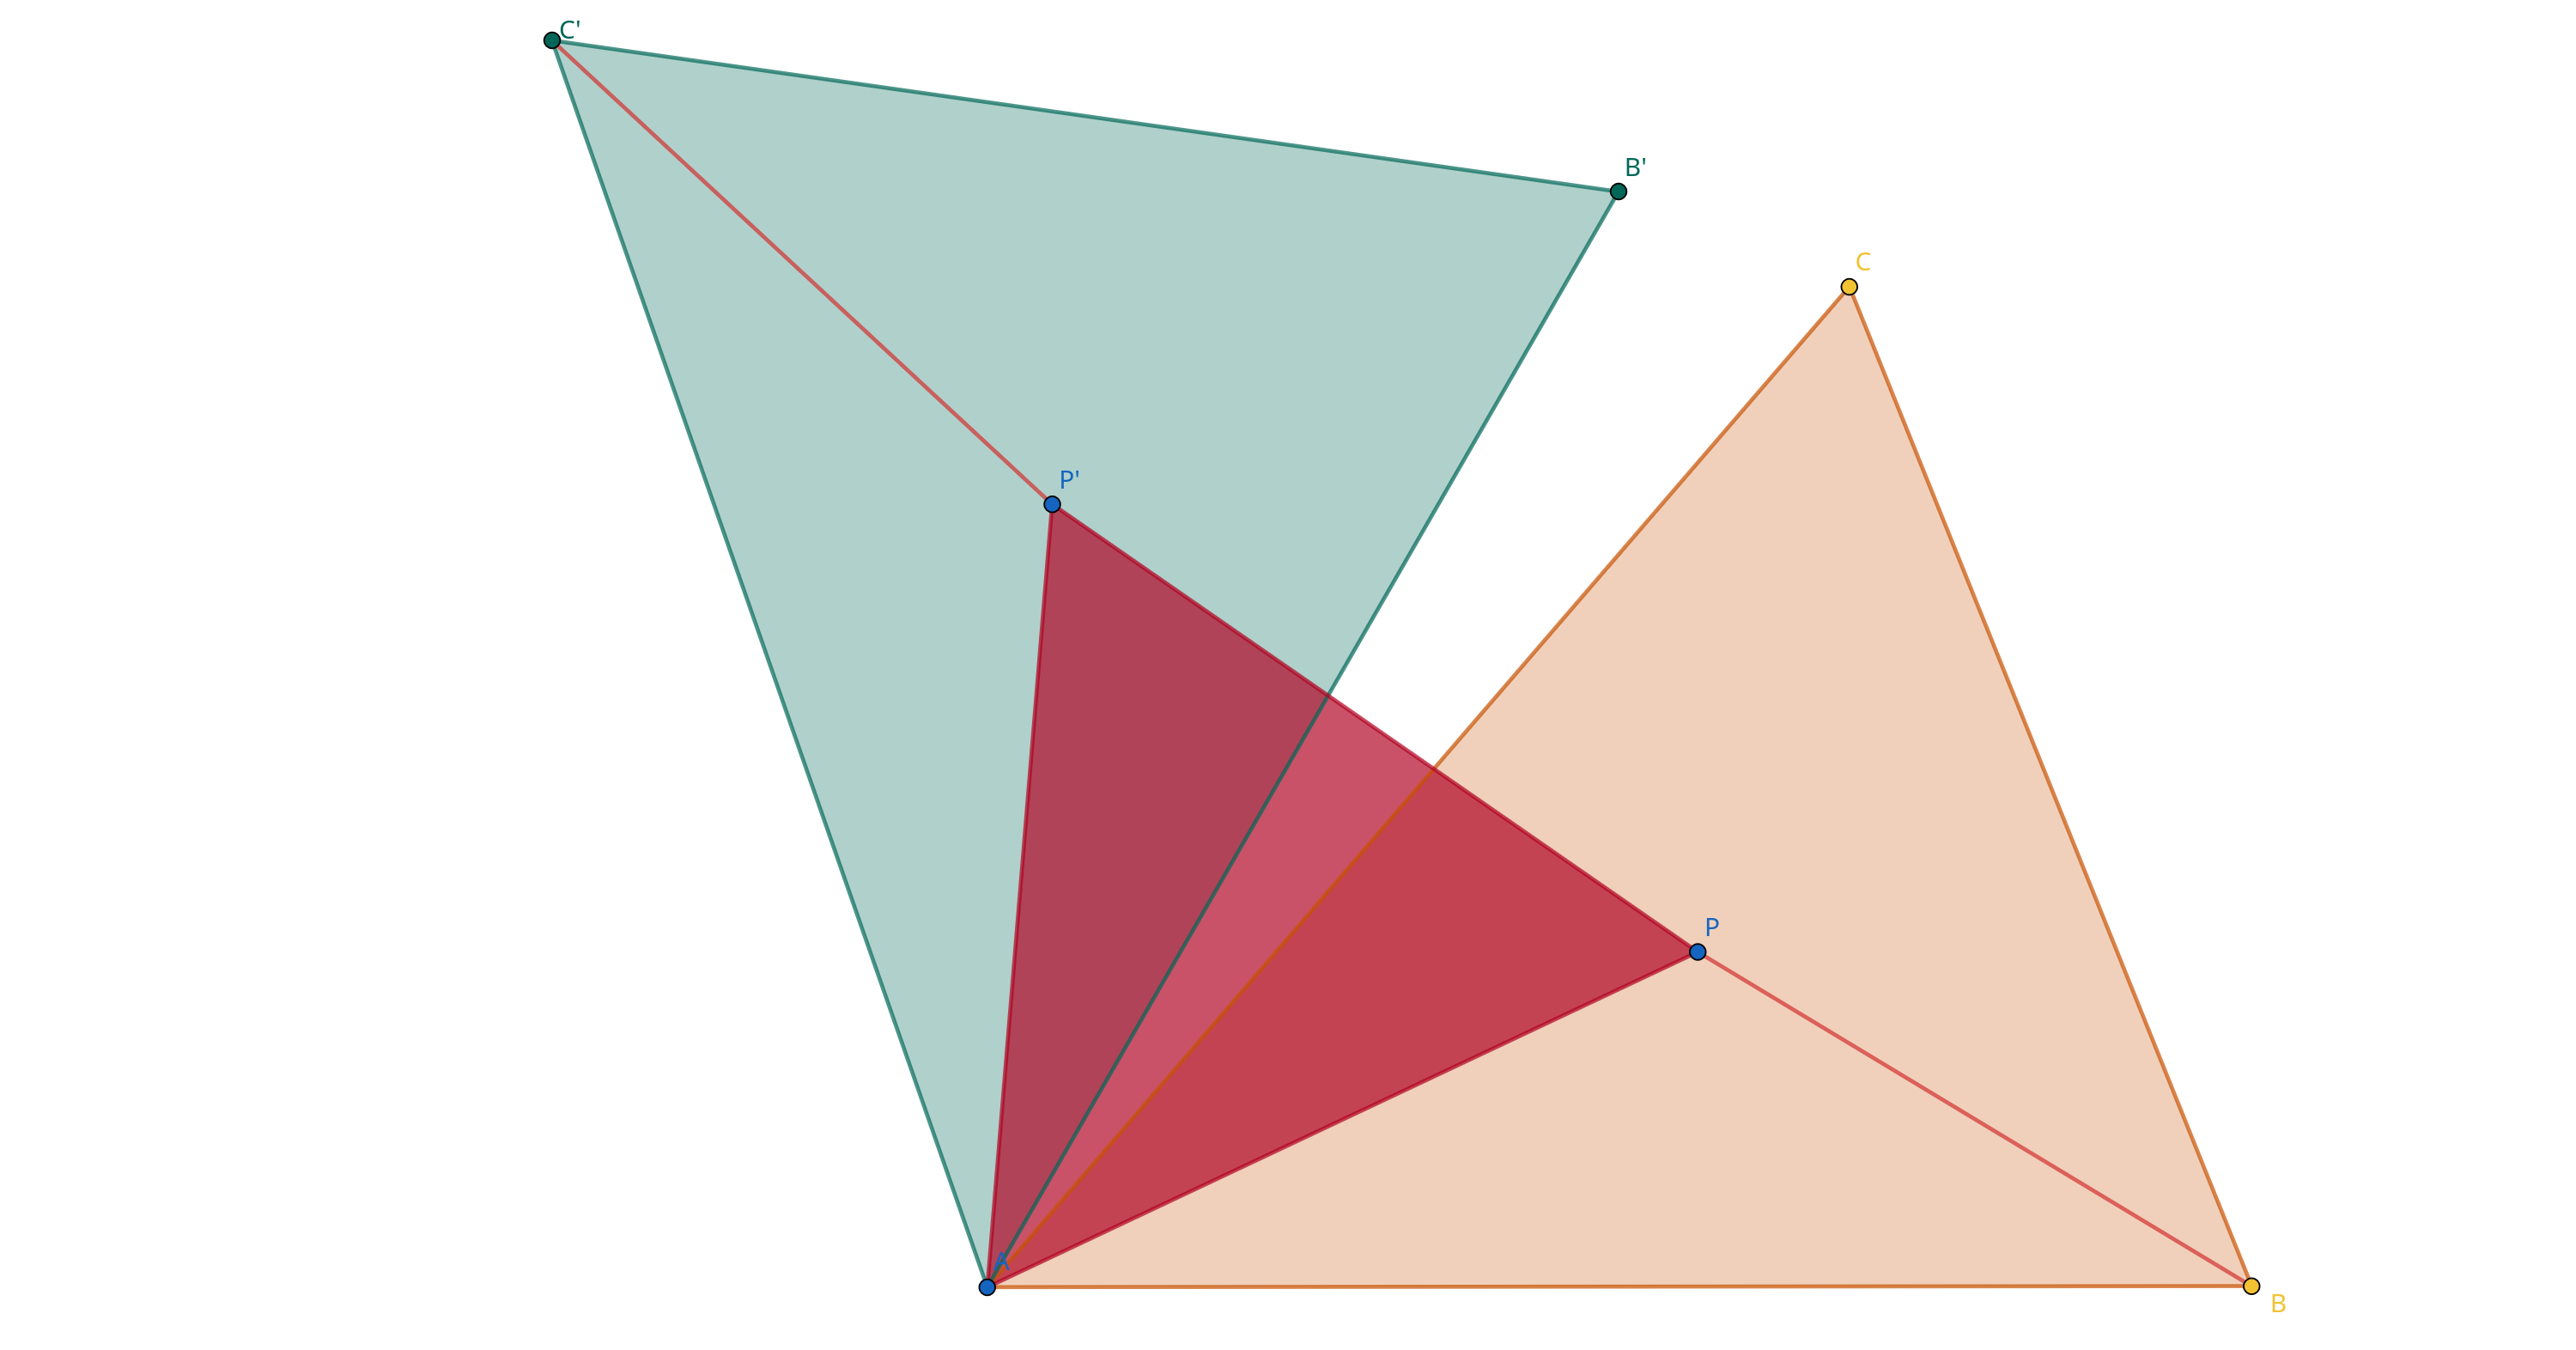
\includegraphics[width=0.8\textwidth]{Blatt05_Aufgabe_15.png}
    \caption{Skizze}
    \label{fig:mein_bild}
\end{figure}
\noindent Seien A, B, C Punkte und $\triangle ABC$ ein Dreieck, bei dem jeder Innenwinkel $< 120\degree$ ist. Sei P ein beliebiger Punkt in der Ebene. Seien B', C' und P' die Bilder von B, C und P, wenn man diese um $60\degree$ gegen den Uhrzeigersinn um A dreht.
Drehung um einen Punkt erhalten Abstände, damit ist $\triangle APP'$ ein gleichseitiges Dreick, denn:
\begin{align*}
    & \angle PAP' = 60\degree \quad \text{und} \quad |AP| = |AP'| \\
    & \Rightarrow \angle PAP' = \angle AP'P = \angle P'PA = 60\degree
\end{align*}
Analog ist das Dreieck $\triangle ACC'$ auch gleichseitig.\\
Die Dreiecke $\triangle APC$ und $\triangle AP'C'$ sind kongruent nach SWS, denn Drehungen um einen Punkt erhalten auch Winkel:
\begin{align}
    & |AP| = |AP'| \quad \text{und} \quad |AC| = |AC'| \\
    & \angle APC = \angle AP'C'
\end{align}
Da $\triangle APP'$ gleichseitig und die Drehung um einen Punkt Abstände erhält, gilt:
\begin{align*}
    & |AP| = |PP'| \quad \text{und} \quad |C'P'| = |CP| \\
    & \Rightarrow |AP| + |BP| + |CP| = |C'P'| + |P'P| + |PB|
\end{align*}
Der Abstand $|C'P'| + |P'P| + |PB|$ ist minimal, wenn die Punkte C', P', P und B auf einer Geraden liegen. Also:
\[
    \angle C'P'P = \angle P'PB = 180\degree
\]
Da $\triangle APP'$ ein gleichseitiges Dreieck ist gilt $\angle AP'P = \angle PP'A = 60 \degree$. Nach der Winkelsumme im Kreis, Kongruenz von $\triangle APC$ und $\triangle AP'C'$ und $\angle C'P'P = \angle P'PB = 180 \degree$ folgt: 
\[
    360\degree - 180\degree - 60\degree = 120 \degree = \angle APB = \angle AP'C' = \angle APC = \angle BPC
\]
\newpage
\noindent Also ist $|AP| + |BP| + |CP|$ minimal, wenn die Winkel $\angle APB = \angle BPC = \angle CPA = 120\degree$ betragen. Die Voraussetzung, dass alle Innenwinkel des Dreiecks $< 120^\circ$ sind, stellt sicher, dass der Punkt $P$ mit den Winkelbedingungen $\angle APB = \angle BPC = \angle CPA = 120^\circ$ tatsächlich im Inneren des Dreiecks existiert. Ist ein Innenwinkel $\geq 120^\circ$, so liegt das Minimum der Abstandssumme in dieser Ecke und nicht im Inneren, und die obige Konstruktion ist dann nicht mehr möglich.

\subsection*{Zusatz}
Seien \(A, B, C \in \mathbb{R}^2\) feste, nicht kollineare Punkte und sei \(f: \mathbb{R}^2 \to \mathbb{R}\) definiert durch 
\[     
    f(P) = |PA| + |PB| + |PC|, 
\] 
Für einen festen Punkt \(Q \in \mathbb{R}^2\) ist die Funktion 
\[     
    g(P) = |P - Q| 
\] 
auf ganz \(\mathbb{R}^2\) konvex. Dies folgt unmittelbar aus der Dreiecksungleichung: Für alle \(P_1, P_2 \in \mathbb{R}^2\) und \(\lambda \in [0,1]\) gilt 
\[     
    | \lambda P_1 + (1-\lambda) P_2 - Q | \leq \lambda |P_1 - Q| + (1-\lambda) |P_2 - Q|. 
\] 
Damit ist \(g\) konvex, aber nicht streng konvex auf Geraden durch \(Q\), da dort die Funktion linear verläuft. Die Summe endlich vieler konvexer Funktionen ist wieder konvex. Streng konvex ist die Summe, wenn mindestens einer der Summanden streng konvex ist und die anderen nicht linear in dieselbe Richtung verlaufen. Im Fall von drei nicht-kollinearen Punkten \(A, B, C\) ist die Funktion 
\[     
    f(P) = |PA| + |PB| + |PC| 
\] 
auf ganz \(\mathbb{R}^2\) sogar streng konvex, da es keine Gerade gibt, auf der alle drei Summanden gleichzeitig linear sind. 
Daraus folgt: \(f\) besitzt genau ein Minimum in \(\mathbb{R}^2\), das heißt, es existiert eindeutig ein Punkt \(P\), der die Summe der Abstände zu den drei Ecken minimal macht.
\end{document}
